% \documentclass[12pt,english]{article}
\documentclass[titlepage]{article}
\usepackage[T1]{fontenc}
\usepackage{amsmath}
\usepackage{babel}
\usepackage{graphicx}
\graphicspath{{../images/}}

% widen margins
\usepackage[margin=1in]{geometry}


\author{
    Meisel, Carlos \\
  \and
  Juarez, Albert\\
  \and
    Quintero, Osvaldo\\
}
\title{Task 6 - OLVHN}
\begin{document}
  \maketitle

  \tableofcontents

\section{Overview}
This report contains the results and summary of the 12 step process described in Dr. Cizmas notes for computing the Operating Line. 
Also included in this report is the engine performance vartiatio with wheel speed, altitude and aircraft speed.

\section{Methodology for Computing the Operating Line}
As  we determine the Operating Line of our engine, we first define our 
operating parameters:

\begin{equation}
  \dot{m}_{air} = 1.64089 \left[\frac{kg}{s} \right]
\end{equation}

\begin{equation}
  w_{c_{n}} = 283.91025 \left[\frac{kJ}{kg}\right]
\end{equation}

\begin{equation}
  \eta_{compressor_{n}} = 0.90
\end{equation}

\begin{equation}
  \sigma_{comb} = 0.90
\end{equation}

\begin{equation}
  \eta_{turbine} = 0.94
\end{equation}

\begin{equation}
  \pi_{c_{n}} = 9.2
\end{equation}

\begin{equation}
  \lambda = 2.85377
\end{equation}

\begin{equation}
  T_{1_{n}}^{*} = 288.16 [K]
\end{equation}

\begin{equation}
  T_{3_{n}}^{*} = 1410 [K]
\end{equation}

\begin{equation}
  p_{1_{n}}^{*} =  1.01325 [bar]
\end{equation}

\begin{equation}
  p_{3_{n}}^{*} =  9.042243 [bar]
\end{equation}

\begin{equation}
  h_{3_{n}}^{*} =  1574.3477 \left[\frac{kJ}{kg}\right]
\end{equation}

\begin{equation}
  N_{n} = 52612.464822 [rpm]
\end{equation}

\begin{equation}
  \pi_{D} = 0.93
\end{equation}

\begin{equation}
  \gamma_{g} = 1.304286
\end{equation}

\begin{equation}
  \frac{A_{3.5}}{A_{5}} = 1.2
\end{equation}

\begin{equation}
  h_{1}^{*} = 288.299988 \left[\frac{kJ}{kg}\right]
\end{equation}

\begin{enumerate}
  \item Calculate the compressor work $w_{c}$, given an angular speed calculated
  in Task2, as a function of nominal compressor work and nominal angular speed.

  \begin{equation}
    w_{c} = w_{c_{n}} \left( \frac{N}{N_{n}} \right)^{x}
  \end{equation}
  Usually $x \in [1.9, 2.1]$, for convience we will start with $x = 2.1$.

  Note: 

  \begin{equation}
    N = 1.1N_{r}
  \end{equation}

  Recall when at nominal conditions:

  \begin{equation}
    N_{r} = \frac{N_{n}}{1.05}
  \end{equation}

  \begin{center}
    \begin{tabular}{|c|c|}
      \hline
      $N$ & $w_{c}$ \\
      \hline
      55117.82029 rpm & 313.0460185$\frac{kJ}{kg}$ \\
      \hline
    \end{tabular}
  \end{center}

  \item Estimate the compressor efficiency $\eta_{c}$, given an angular 
  speed calculated in Task2, as a function of nominal compressor efficiency and
  nominal angular speed. We start by calculated the pressure ratio $\pi_{c}^{*}$

  \begin{equation}
    \pi_{c}^{*} = \left[ \left(\pi_{c_{n}}^{\frac{\gamma-1}{\gamma}}\right)
    \frac{\eta_{c}}{\eta_{c_{n}}} \left(\frac{N}{N_{n}}\right)^{x} +1 \right]^{\frac{\gamma}{\gamma-1}}
  \end{equation}

  To begin the caluation we can start by assuming $\eta_{c} = \eta_{c_{n}}$. Once
  the pressure ratio is calculated, read that $\pi_{c}^{*}$ from the compressor map, 
  and find the corresponding $\dot{m}\frac{\sqrt{T_{1}^{*}}}{p_{1}^{*}}$. Once you have 
  that, find the corresponding $\eta_{c}$ from the compressor map. If $\eta_{c} \neq \eta_{c_{n}}$ 
  then iterate until the change is less than a allowed tolerance. For our engine,
  we allowed a tolerance of $0.01$.

  \begin{center}
    \begin{tabular}{|c|c|}
      \hline
      $\pi_{c}^{*}$ & $\eta_{c}$ \\
      \hline
      10.4001622 & 0.878213 \\
      \hline
    \end{tabular}
  \end{center}
  \item Calculate the $T_{3}^{*}$ from:
  
  \begin{equation}
    \pi_{c}^{*} = \frac{1+f}{\sigma_{comb}} \left( \frac{p_{3}^{*}}{\dot{m}\sqrt{T_{3}^{*}}} \right)_{n}
    \sqrt{\frac{T_{3}^{*}}{T_{1}^{*}}} \frac{\dot{m}\sqrt{T_{1}^{*}}}{p_{1}^{*}}
  \end{equation}
  Where:
  \begin{equation}
    \frac{1+f}{\sigma_{comb}} \left( \frac{p_{3}^{*}}{\dot{m}\sqrt{T_{3}^{*}}} \right)_{n} = constant
  \end{equation}
  
  From here, calculate $h_{3}^{*}$ from:

  \begin{equation}
    h_{3}^{*} = \left(\frac{1+minL}{1+\lambda minL}\right) h_{\lambda =1} + \left(\frac{(\lambda -1) minL}{1+\lambda minL}\right) h_{air}
  \end{equation}

  Where:
  \begin{itemize}
    \item $h_{\lambda}$ - enthalpy of the combustion products for $\lambda$ excess air
    \item $h_{\lambda = 1}$ - enthalpy of the combustion products for stoichiometric combustion
    \item $h_{air}$ - enthalpy of the air
  \end{itemize}

  Check to see if the ratio $\frac{w_{c}}{h_{3}^{*}}$ is equal to the nominal ratio
  $\frac{w_{c_{n}}}{h_{3_{n}}^{*}}$. If not, iterate x until it is, within a reasonable tolerance of about 1\%.

  \vspace{0.5cm}

  After iterating x, we arrived to $x = 1.4$.

  \begin{center}
    \begin{tabular}{|c|c|}
      \hline
      $T_{3}^{*}$ & $h_{3}^{*}$ \\
      \hline
      1552.103717 [K] & 1753.74986 $\frac{kJ}{kg}$ \\
      \hline
    \end{tabular}
  \end{center}

  \item We are now to find the critical conditions by:
  
  \begin{equation}
    \pi_{c_{cr}}^{*} = \frac{1}{\sigma_{comb} \pi_{D}} \left[ \frac{\frac{\gamma_{g}+1}{2}}{1 - \frac{w_{c}}{h_{3}^{*}} \frac{1}{\eta_{turbine}}} \right]^{\frac{\gamma_{g}}{\gamma_{g}-1}}
  \end{equation}

  \begin{equation}
    N_{cr} = N_{n} \sqrt{\frac{\eta_{c_{n}}}{\eta_{c_{cr}}}} \frac{\pi_{c_{cr}}^{\frac{\gamma - 1}{\gamma}} -1}{\pi_{c_{n}}^{\frac{\gamma -1}{\gamma}} - 1}
  \end{equation}

  We are to then repeat steps (1)-(3) for three values of angular speed
  larger than the critical angular speed.

  \begin{center}
    \begin{tabular}{|c|c|c|}
      \hline
      $\pi_{c_{cr}}^{*}$ & $N_{cr}$ & $\eta_{c_{cr}}$ \\
      \hline
      5.462985 & 44711.24058 rpm & 0.879 \\
      \hline
    \end{tabular}
  \end{center}

  \begin{center}
    \begin{tabular}{|c|c|c|}
      \hline
      $\frac{w_{c}}{h_{3}^{*}}$ & $\left(\frac{w_{c}}{h_{3}^{*}}\right)_{n}$ & \% diff \\
      \hline
      0.1785009519 & 0.180335162 & 1.0171116 \% \\
      \hline
    \end{tabular}
  \end{center}

  Now we repeat steps (1)-(3) for three values of angular speed larger than the critical angular speed.

  \begin{center}
    \begin{tabular}{|c|c|c|c|c|c|c|c|c|}
      \hline
      $N$ & $w_{c}$ & $\eta_{iteration}$ & $\pi_{c}^{*}$ & $\bar{m}$ \\
      \hline
      46946.803 & 223.4949 & 0.881 & 6.17351 & 0.71 \\
      \hline
      49182.365 & 246.4306 & 0.879 & 7.09622 & 0.785 \\
      \hline
      51417.93	& 270.5425 & 0.9	& 8.5075	& 0.9 \\
      \hline
    \end{tabular}
  \end{center}

  \begin{center}
    \begin{tabular}{|c|c|c|c|c|}
      \hline
      $N$ & $T_{3}^{*}$ & $h_{3}^{*}$ & $\frac{w_{c}}{h_{3}^{*}}$ & \% diff \\
      \hline
      46946.803 & 1150.965 & 1251.825 & 0.17854 & 0.998 \\
      \hline
      49182.365 & 1244.026485 & 1368.077 &	0.18013	& 0.1142 \\
      \hline
      51417.93 & 1360.3106 & 1512.1349	& 0.1789	& 0.7879 \\
      \hline
    \end{tabular}
  \end{center}


  \item Once we have reached the critical value, our ratio $\frac{w_{c}}{h_{3}^{*}}$ is no longer constant. If the flow isn't critical,
  then the variation of $\frac{w_{c}}{h_{3}^{*}}$ is given by:

  \begin{equation}
    \frac{w_{c}}{h_{3}^{*}} = \eta_{turbine} \left[ 1 - \left(\frac{p_{H}}{p_{3}^{*}}\right)^{\frac{\gamma_{g}-1}{\gamma_{g}}} - K \left(\frac{A_{3.5}}{A_{5}}\right)^{2} \left(\frac{p_{3}^{*}}{p_{H}}\right)^{\frac{2}{\gamma_{g}}} \right] 
  \end{equation}
  
  Where:

  \begin{equation}
    K = \left(\frac{A_{5}}{A_{3.5}}\right)^{2} \left(\frac{p_{H}}{p_{3}^{*}}\right)^{\frac{2}{\gamma_{g}}}\left[1 - \left(\frac{p_{H}}{p_{3}^{*}}\right)^{\frac{\gamma_{g}-1}{\gamma_{g}}} \frac{w_{c}}{h_{3}^{*}} \frac{1}{\eta_{turbine}}\right] 
  \end{equation}

  \begin{equation}
    \frac{p_{H}}{p_{3}^{*}} = \frac{1}{\sigma_{combustion}^{*} \pi_{c}^{*} \pi_{D}}
  \end{equation}

  Recall that $\pi_{D}$ is given by:

  \begin{equation}
    \pi_{D} = \frac{p_{1}^{*}}{p_{H}}
  \end{equation}

  When performing this step be sure to choose a $\pi_{c}^{*}$ that is less than the critical value $\pi_{c_{cr}}^{*}$.

  \begin{center}
    \begin{tabular}{|c|c|c|}
      \hline
      $K$ & $\frac{p_{H}}{p_{3}^{*}}$ & $\frac{w_{c}}{h_{3}^{*}}$ \\
      \hline
      0.007177101 & 0.23020826 & 0.180335162\\
      \hline
    \end{tabular}
  \end{center}

  \item Now we are to choose an $N$ value smaller than the critical value $N_{cr}$, and calculate $w_{c}$ using equation (16)
  We chose a $N$ value that was 1\% less than the critical value.

  \begin{equation}
    N < N_{cr}
  \end{equation}

  Now we use equation (16) to calculate $w_{c}$. 

  \begin{center}
    \begin{tabular}{|c|c|}
      \hline
      $N$ & $w_{c}$ \\
      \hline
      44500 rpm & 199.73351054474077 $\frac{kJ}{kg}$ \\
      \hline
    \end{tabular}
  \end{center}

  \item Now calculate $h_{3}^{*}$ from equation (26) and $w_{c} = 171.430154 \frac{kJ}{kg}$.
  
  \begin{equation}
    h_{3}^{*} = w_{c_{n}} \left( \frac{w_{c}}{h_{3}^{*}}\right)^{-1}
  \end{equation}

  \begin{center}
    \begin{tabular}{|c|}
      \hline
      $h_{3}^{*}$ \\
      \hline
      1107.56831 $\frac{kJ}{kg}$ \\
      \hline
    \end{tabular}
  \end{center}

  \item Calculate $T_{3}^{*}$ using the stoichiometric and air gas tables. 
  
  \begin{center}
    \begin{tabular}{|c|}
      \hline
      $T_{3}^{*}$ \\
      \hline
      1028.878066 K \\
      \hline
    \end{tabular}
  \end{center}

  \item For known value of $\pi_{c}^{*}$ and $N$ read from the the compressor map the value of the corrected mass flow rate

  \begin{equation}
    \pi{_c}^{*} = 5.18983611172067
  \end{equation}

  Yields a corrected mass flow rate of:

  \begin{center}
    \begin{tabular}{|c|}
      \hline
      $m_{a}\frac{\sqrt{T_{1}^{*}}}{p_{1}^{*}}$ \\
      \hline
      (0.63)(1.6087157)$\frac{\sqrt{288}}{101325}$ \\
      \hline
    \end{tabular}
  \end{center}

  \item Now determine $T_{3}^{*}$ using equation (21).
  \item Compare the values of $T_{3}^{*}$ from step 8 to $T_{3}^{*}$ from step 10, if they differ by more than 10 degrees K, then iterate until with different $N$ value.
  
  \begin{center}
    \begin{tabular}{|c|}
      \hline
      $T_{3}^{*}$ \\
      \hline
      1033.097120243129 K \\
      \hline
    \end{tabular}
  \end{center}

\item Now choose another value of $\pi_{c}^{*}$ and go back to step 5 and repeat the process to get other points on the operating line at $\frac{p_{H}}{p_{3}^{*}}$ 

\begin{center}
  \begin{tabular}{|c|c|c|c|c|c|}
    \hline
    $\pi_{c}^{*}$ & $\frac{p_{H}}{p_{3}^{*}}$ & $K$ & $\frac{w_{c}}{h_{3}^{*}}$ & $N$ \\
    \hline
    6.009283919	& 0.198816223	& 0.007124393 &	0.180335162	& 44500 \\
    \hline
    7.101880995	& 0.168229112 &	0.006698233 &	0.180335162	& 40000 \\
    \hline
    8.194478071 &	0.145798563 &	0.006163854	& 0.180335162	& 50000 \\
    \hline
  \end{tabular}
\end{center}

\begin{center}
  \begin{tabular}{|c|c|c|c|}
    \hline
    $w_{c}$ & $h_{3}^{*}$ & $T_{3}^{*}$ & $T_{3}^{*}$ \\
    \hline
    199.73351054474077	& 1107.56831	& 1028.878066	& 1033.097120243129 \\
    \hline
    159.6691061	& 885.4019626 &	839.0287095 & 833.1424783 \\
    \hline
    255.1126073	& 1414.658156	& 1281.631036 & 1276.178685 \\
    \hline
  \end{tabular}
\end{center}



\end{enumerate}

\begin{figure}[h]
  \centering
  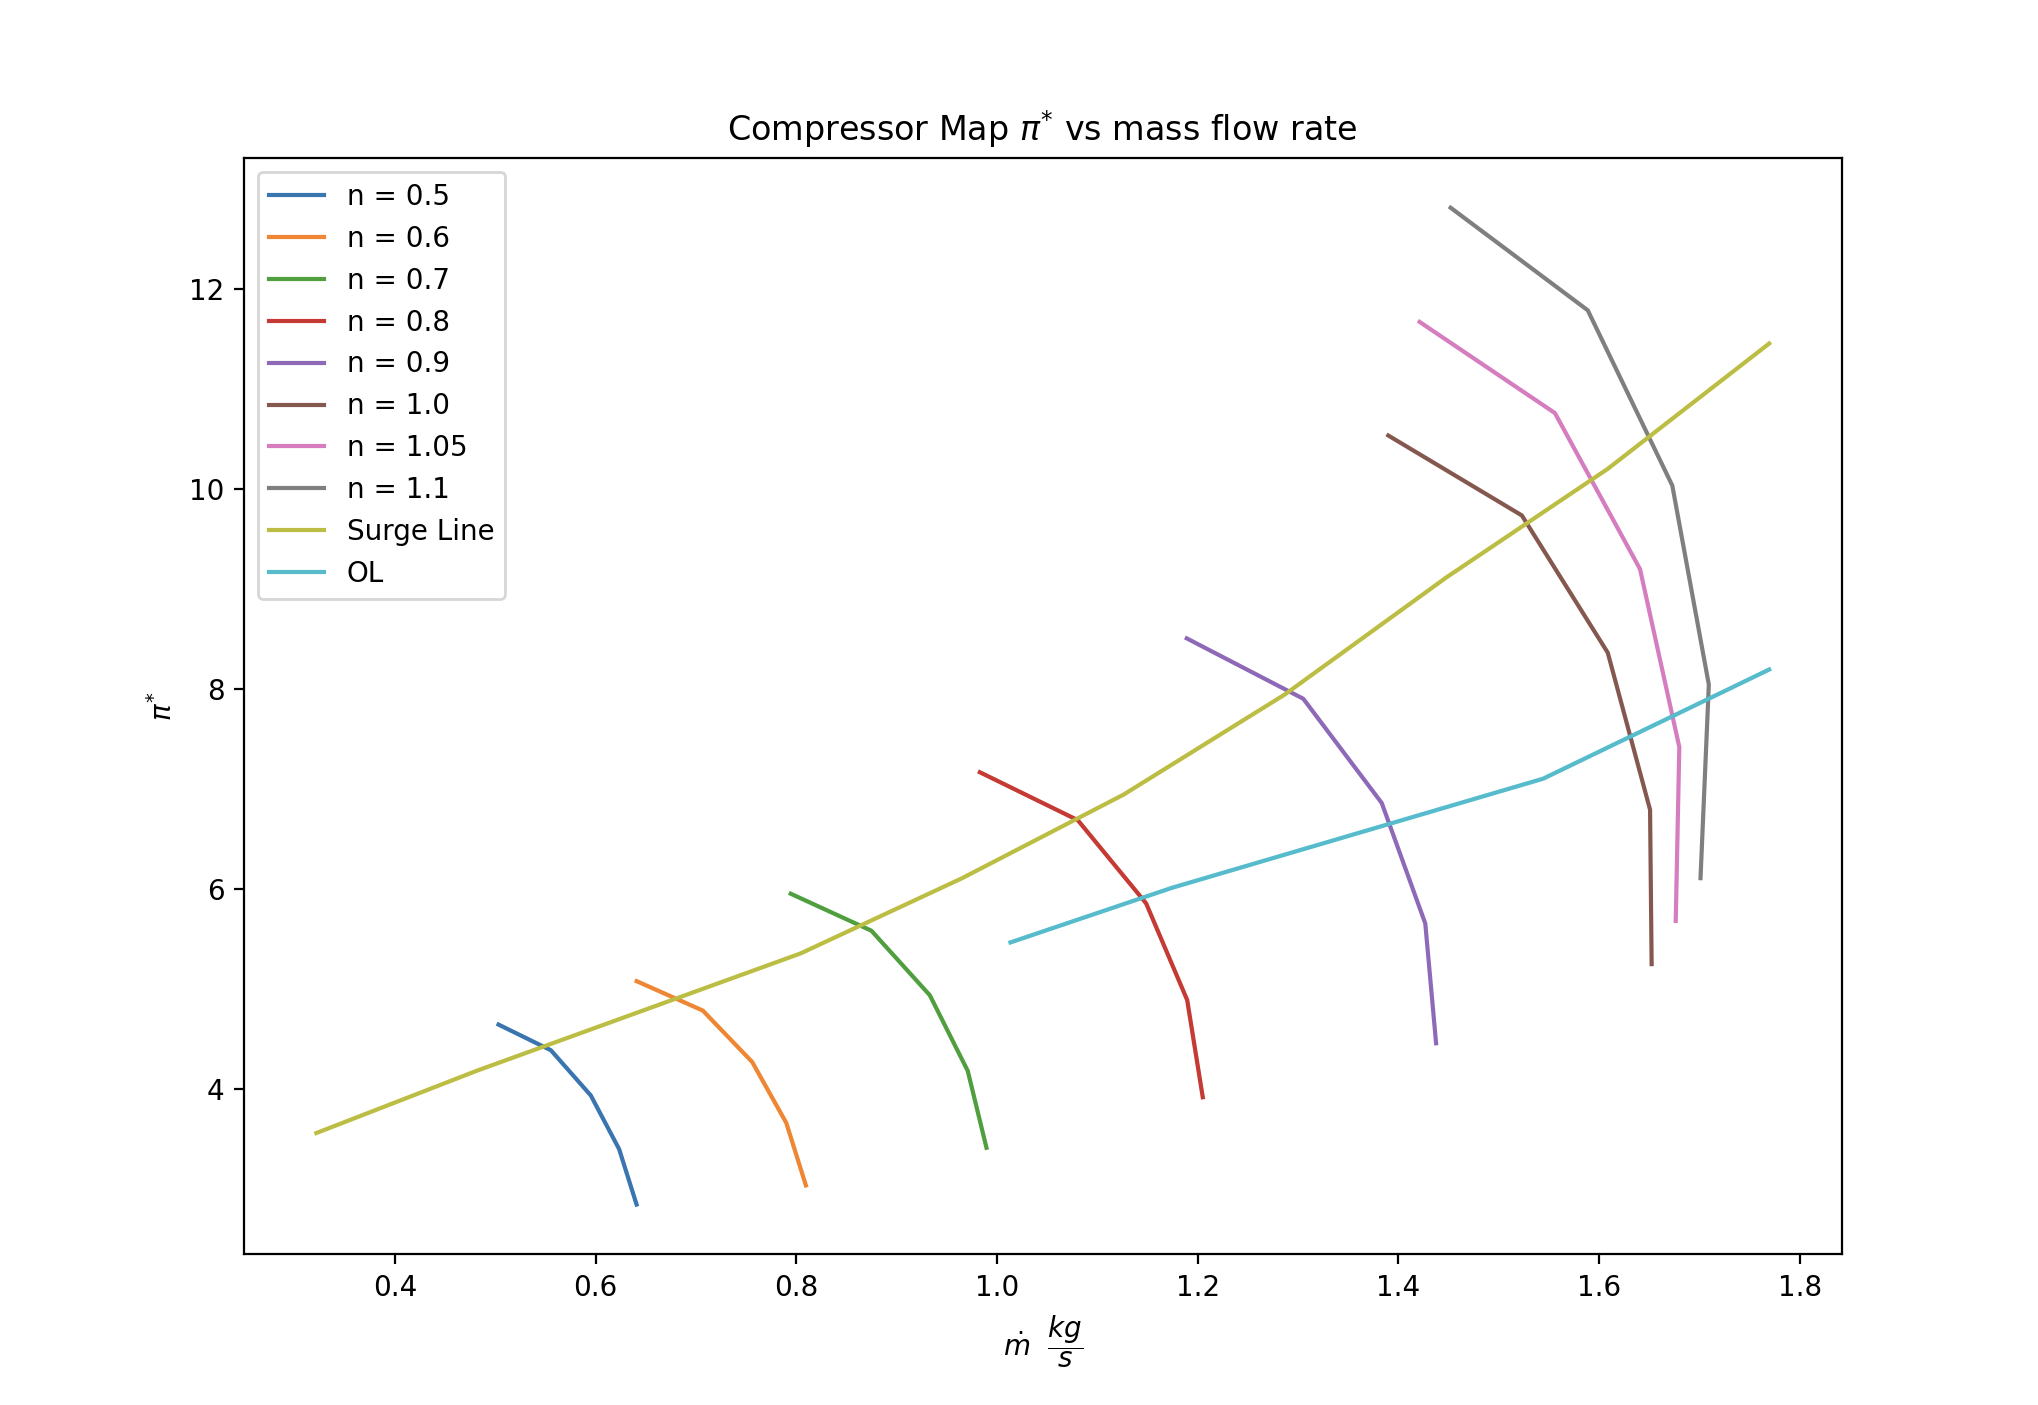
\includegraphics[width=\textwidth]{CompressorMap.png}
  \caption{Compressor Map with Surge Line and Operating Line (OL)}
  \label{fig:CompressorMap}
\end{figure}

\vspace{2cm}

\begin{section}{Jet Engine Performance Variation with Wheel Speed}

To determine the performance variation with wheel speed (N) we are to use the \textbf{Operating Line} from Section 2. We will choose wheel speeds that are different 
from the nominal wheel speed $N_{n}$, and then read from the Compressor Map the pressure ratios $\pi_{c}^{*}$ and the efficiencies $\eta_{c}$.

\begin{center}
  \begin{tabular}{|c|c|c|}
    \hline
    $N$ & $\pi_{c}^{*}$ & $\eta_{c}$ \\
    \hline
    40000 rpm & 7.101880995 & 0.849 \\
    \hline
    44500 rpm & 6.009283919 & 0.877 \\
    \hline
    49000 rpm & 7.9900312 & 0.8325 \\
    \hline
  \end{tabular}
\end{center}

Now similar to how we solved for compressor work, we make use of equation (17):

\begin{center}
  $$w_{c} = w_{c_{n}} \left( \frac{N}{N_{n}}\right)^{x}$$
\end{center}

Here we will use $x = 2$ following Dr. Cizmas' Example.

\begin{center}
  \begin{tabular}{|c|}
    \hline
    $w_{c}$ \\
    \hline
    203.1064891\\
    \hline
    164.1057354 \\
    \hline
    246.2611692 \\
    \hline
  \end{tabular}
\end{center}

The enthalpy at stage 02 is calculated:

\begin{equation}
  h_{2}^{*} = h_{1}^{*} + w_{c}
\end{equation}

\begin{center}
  \begin{tabular}{|c|}
    \hline
    $h_{2}^{*}$ \\
    \hline
    491.4064771 \\
    \hline
    452.4057234 \\
    \hline
    534.5611572 \\
    \hline
  \end{tabular}
\end{center}

The degree of dynamic compression in the inlet nozzle is recalculated as:

\begin{equation}
  \pi_{D} = \sigma_{inlet}^{*} \left( 1+\frac{\gamma - 1}{2}M_{H}^{2}\right)^{\frac{\gamma}{\gamma - 1}}
\end{equation}

Recall $\sigma_{inlet}^{*} = 0.93$. Also here we are assuming $M_{H} = 0$, since we are at Take-off conditions.

\begin{center}
  \begin{tabular}{|c|}
    \hline
    $\pi_{D}$ \\
    \hline
    0.93 \\
    \hline
    0.93 \\
    \hline
    0.93 \\
    \hline
  \end{tabular}
\end{center}

The specific thrust is now recalculated as:

\begin{equation}
  F_{sp} = \phi \sqrt{2h_{3}^{*}\left[1 - \frac{1}{\pi_{D} \pi_{c}^{*} \sigma_{comb}^{*}}\right]^{\frac{\gamma_{g}-1}{\gamma_{g}}} - h_{1}^{*}\left(\frac{\pi_{c}^{\frac{\gamma-1}{\gamma}}}{\eta_{c}}\right)} \left(1+\frac{1}{\lambda minL}\right)
\end{equation}

\begin{center}
  \begin{tabular}{|c|c|c|c|c|}
    \hline
    $F_{sp}$ & $\frac{p_{H}}{p_{3}^{*}}$ & $K$ & $\frac{w_{c}}{h_{3}^{*}}$ & $h_{3}^{*}$ \\
    \hline
    731.102889 & 0.198816223	& 0.007124393 &	0.180335162	& 1126.272254 \\
    \hline
    656.888117 & 0.168229112	& 0.006698233	& 0.180335162	& 910.0040937 \\
    \hline
    875.895256 & 0.149529804 & 0.006265198	& 0.180335162	& 1365.574893 \\
    \hline
  \end{tabular}
\end{center}

The mass flow rate is recalculated as:

\begin{equation}
  \dot{m}_{air} = \dot{m}_{air_{n}} \frac{\pi{c}^{*}}{\pi_{c_{n}}^{*}} \frac{N_{n}}{N}
\end{equation}

\begin{center}
  \begin{tabular}{|c|}
    \hline
    $\dot{m}_{air}$ \\
    \hline
    1.26719369 \\
    \hline
    1.666071704 \\
    \hline
    1.530139367 \\
    \hline
  \end{tabular}
\end{center}

And the TSFC is recalculated as:

\begin{equation}
  TSFC = \frac{3600}{F_{sp}} \frac{1}{\lambda minL}
\end{equation}

\begin{center}
  \begin{tabular}{|c|}
    \hline
    TSFC \\
    \hline
    0.117699 \\
    \hline
    0.130996 \\
    \hline
    0.098242 \\
    \hline
  \end{tabular}
\end{center}

\begin{figure}[h]
  \centering
  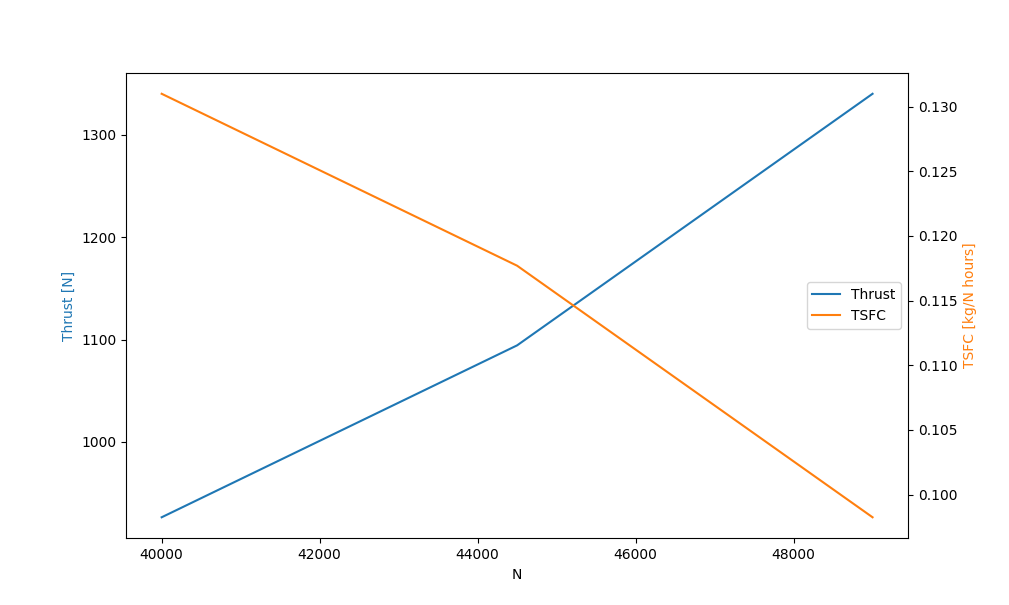
\includegraphics[width=\textwidth]{fig_N.png}
  \caption{Engine performance variation with wheel speed}
  \label{fig:WheelSpeedVar}
\end{figure}

\vspace{7cm}

Above is the the plot of the engine performance variation with wheel speed $N$ [rpm]

\end{section}

\section{Jet Engine Performance Variation with Altitude and Speed}

Up to this point, our engine has been performance has been calculate at take-off conditions. It is very important for us to determine how the 
performance varies with altitude and speed. 

\begin{enumerate}
  \item First we are to calculate the Mach number at H and V.
  
  \begin{equation}
    M_{H} = \frac{V}{\sqrt{\gamma R T_{H}}}
  \end{equation}

  It is important for us to specify our altitude dependent properties and speed dependent properties.

  \begin{center}
    \begin{tabular}{|c|c|c|c|}
      \hline
      $H$ [m] & $T_{H}$ [K] & $p_{H}$ [Pa] & $a_{H}$ [m/s] \\
      \hline
      0 & 288.15 & 101325 & 340.29 \\
      \hline
      1000 & 281.65 & 89874.6	& 336.434 \\
      \hline
      3000	& 268.65	& 70108.5	& 328.578 \\
      \hline
      5000	& 255.65	& 54019.9	& 320.529 \\
      \hline
      6000	& 249.15	& 47181 &	316.428 \\
      \hline
      7000 &	242.65	& 41060.7	& 312.274 \\
      \hline
      8000	& 236.15	& 35599.8	& 308.063 \\
      \hline
      9000	& 229.65	& 30742.5 &	303.793 \\
      \hline
      10000	& 223.15	& 26436	& 299.463 \\
      \hline
    \end{tabular}
  \end{center}

  And our velocity values:

  \begin{center}
    \begin{tabular}{|c|}
      \hline
      $v$ [m/s] \\
      \hline
      0 \\
      \hline
      100 \\
      \hline
      200 \\
      \hline
      300 \\
      \hline
      350 \\
      \hline
      400 \\
      \hline
    \end{tabular}
  \end{center}

  \item Now one can calculate the degree of dynamic compression $\pi_{D}$.
   \begin{equation}
      \pi_{D} = \frac{p_{1}^{*}}{p_{H}} = \sigma_{inlet}^{*} \frac{p_{H}^{*}}{p_{H}}
   \end{equation}


   This means that we can say:
   \begin{equation}
    \pi_{D} = \sigma_{inlet}^{*} \left(1+\frac{\gamma-1}{2} M_{H}^{2}\right)^{\frac{\gamma}{\gamma-1}}
   \end{equation}

   Where $\sigma_{inlet}^{*}$ is the inlet stagnation pressure loss in the inlet defined as the ratio between the stagnation pressure at the inlet
   in the compressor $p_{1}^{*}$ and the stagnation pressure at the inlet of the engine $p_{H}$.

   \begin{center}
    \begin{tabular}{c c c c c c c c c c c }
      \hline
      \textbf{$H$ [km]} & 0 & 1 & 3 & 5 & 6 & 7 & 8 & 9 & 1 & \textbf{$v$ [m/s]} \\
      \hline
      \textbf{$\pi_{D}$} & 0.93 &	0.93	& 0.93	& 0.93	& 0.93 &	0.93 & 	0.93 & 	0.93 & 	0.93 & 0 \\
      \hline
      \textbf{$\pi_{D}$} & 0.9889	& 0.9887	& 0.9917 & 	0.9949	& 0.9966	& 0.9985	& 1.0004 & 	1.0024 &	1.0046 & 100 \\
      \hline
      \textbf{$\pi_{D}$} & 1.1809	&1.1810	&1.1943	& 1.2090	&1.2170	& 1.2254 &	1.2344 &	1.2439 &	1.2541 & 200 \\
      \hline
      \textbf{$\pi_{D}$} &1.5566&	1.5586	&1.5952	&1.6361&	1.6585	&1.6823	&1.7077	&1.7348	&1.7638& 300 \\
      \hline
      \textbf{$\pi_{D}$} &1.8411	&1.8460	&1.9023	&1.9656	&2.0004	&2.0375	&2.0772	&2.1197	&2.1654& 350 \\
      \hline
      \textbf{$\pi_{D}$} &2.2122	&2.2226	&2.3066	&2.4019&	2.4544	&2.5105	&2.5708	&2.6356	& 2.7054& 400 \\
      \hline
    \end{tabular}
  \end{center}

  \item Now we calculate $h_{H}^{*}$.
   \begin{equation}
    h_{H}^{*} = h_{H}\left( 1+ \frac{\gamma-1}{2} M_{H}^{2} \right)
   \end{equation}  

   \item Now calculate the compressor pressure ratio $\pi_{c}^{*}$ with variation of H and V.
   
   \begin{equation}
    \pi_{c}^{*} = \left[ 1+ \frac{h_{0}}{h_{H}^{*}}\left(\pi_{c_{n}}^{* \frac{\gamma-1}{\gamma}} - 1\right) \right] ^{\frac{\gamma}{\gamma-1}}
   \end{equation}

   Students can also calculate $w_{c}$:

   \begin{equation}
    w_{c} = h_{2}^{*} - h_{H}^{*}
   \end{equation}

   \item Now oen can begin calculating the Specific Thrust $F_{sp}$
   \begin{equation}
    F_{sp} = \phi_{5} \sqrt{2h_{3}^{*}\left[1-\frac{1}{(\pi_{D} \pi_{c}^{*} \pi_{combust}^{*})} \right] - h_{1}^{*}}\frac{\pi_{c}^{\frac{\gamma-1}{\gamma}}}{\eta_{c}}\left(1+\frac{1}{\lambda minL}\right) - v
    \end{equation}

  Recall, $\gamma$ varies due to the variance in speed of sound $a$ from the change in altitude.
  
  \begin{equation}
    \gamma = \frac{a_{H}^{2}}{R_{air}T_{H}}
  \end{equation}

  We can calculate $h_{3}^{*}$ similar to previous sections:

  \begin{equation}
    h_{3}^{*} = \left(\frac{w_{c}}{h_{3}^{*}}\right) w_{c}
  \end{equation}
  
  Where $w_{c}$ comes from equation (44) and $\frac{w_{c}}{h_{3}^{*}}$ comes from equations (27), (28), and (29).

  \begin{center}
  
    $\frac{w_{c}}{h_{3}^{*}} = \eta_{turbine} \left[ 1 - \left(\frac{p_{H}}{p_{3}^{*}}\right)^{\frac{\gamma_{g}-1}{\gamma_{g}}} - K \left(\frac{A_{3.5}}{A_{5}}\right)^{2} \left(\frac{p_{3}^{*}}{p_{H}}\right)^{\frac{2}{\gamma_{g}}} \right] $


    $K = \left(\frac{A_{5}}{A_{3.5}}\right)^{2} \left(\frac{p_{H}}{p_{3}^{*}}\right)^{\frac{2}{\gamma_{g}}}\left[1 - \left(\frac{p_{H}}{p_{3}^{*}}\right)^{\frac{\gamma_{g}-1}{\gamma_{g}}} \frac{w_{c}}{h_{3}^{*}} \frac{1}{\eta_{turbine}}\right] $


    $\frac{p_{H}}{p_{3}^{*}} = \frac{1}{\sigma_{combustion}^{*} \pi_{c}^{*} \pi_{D}}$
  \end{center}
  
Now all we have to solve for is the varying $\lambda$. We begin by making use of the energy conservation equation between the inlet and burner.

\begin{equation}
  \dot{m}_{air}h_{2}^{*} + \dot{m}_{fuel} \left(h_{fuel} + \pi_{combust}^{*}LHV\right) = \dot{m}_{air}h_{3}^{*} 
\end{equation}

Recall $LHV = 43.5 \times 10^{6} J/kg$ for standard fuel. We can make use of:

\begin{equation}
  f = \frac{\dot{m}_{fuel}}{\dot{m}_{air}} = \frac{1}{L} = \frac{1}{\lambda minL}
\end{equation}

Resulting in the following equation:

\begin{equation}
  h_{2}^{*} + \frac{\pi_{combust}^{*} LHV}{\lambda minL} = \left[1+ \frac{1}{\lambda minL}\right] h_{3}^{*}
\end{equation}

We have all the necessary variables to solve for $\lambda$, therfore equation (45) can be solved.

\begin{center}
  \begin{tabular}{c c c c c c c c c c c }
    \hline
    \textbf{$H$ [km]} & 0 & 1 & 3 & 5 & 6 & 7 & 8 & 9 & 1 & \textbf{$v$ [m/s]} \\
    \hline
    $F_{sp}$ & 1040	&1002.6	&1032	&1060.84	&1075.03	&1089.1	&1103	&1116.8	&1130.5 & 0 \\
    \hline
    $F_{sp}$ & 938.35	&900.6&	930.9	&960.5	&975.2	&989.6	&1004.01	&1018.3	&1032.5& 100 \\
    \hline
    $F_{sp}$ & 830.5	&792.0	&824.4	&856.4	&872.2	&888.0	&903.7	&919.3	&934.8& 200 \\
    \hline
    $F_{sp}$ & 709.5	&669.3	&705.2	&740.7	&758.3	&775.9	&793.4	&810.9	&828.3& 300 \\
    \hline
    $F_{sp}$ & 641.0	&599.4	&637.4	&675.0	& 693.7	&712.3	&730.8	&749.4	&767.9& 350 \\
    \hline
    $F_{sp}$ & 565.0	&521.5	&562.0	&601.9	&621.7	&641.5	&661.2	&680.9	&700.6& 400 \\
    \hline
  \end{tabular}
\end{center}

One can now calculate $TSFC$:

\begin{equation}
  TSFC = (TSFC)_{n} \frac{F_{sp_{n}}}{F_{sp}} \frac{\lambda_{n}}{\lambda}
\end{equation}



\begin{center}
  \begin{tabular}{c c c c c c c c c c c }
    \hline
    \textbf{$H$ [km]} & 0 & 1 & 3 & 5 & 6 & 7 & 8 & 9 & 1 & \textbf{$v$ [m/s]} \\
    \hline
    $TSFC$ &0.1037	&0.0985	&0.1026	&0.1066	&0.1085	&0.1104	&0.1123	&0.1142	&0.1160& 0 \\
    \hline
    $TSFC$ &0.1120	&0.1066	&0.1108	&0.1149	&0.1168	&0.1187	&0.1206	&0.1225	&0.1243& 100 \\
    \hline
    $TSFC$ &0.1167	&0.1109	&0.1152	&0.1192	&0.1211	&0.1230	&0.1249	&0.1267	&0.1284& 200 \\
    \hline
    $TSFC$ &0.1174	&0.1110	&0.1154	&0.1194	&0.1213	&0.1232	&0.1250	&0.1267	&0.1283& 300 \\
    \hline
    $TSFC$ &0.1163&	0.1094	&0.1139	&0.1180	&0.1199	&0.1218	&0.1235	&0.1252	&0.1268& 350 \\
    \hline
    $TSFC$ &0.1140	&0.1066	&0.1112	&0.1154	&0.1173	&0.1192	&0.1209	&0.1225	&0.1240& 400 \\
    \hline
  \end{tabular}
\end{center}

One can calculate mass flow rate by:

\begin{equation}
  \dot{m_{a}} = \dot{m}_{a_{n}} \frac{\pi_{c}^{*}}{\pi_{c_{n}}^{*}} \frac{p_{H}}{p_{0}} \left( 1+ \frac{\gamma-1}{2}M_{H}^{2}\right)^{\frac{\gamma}{\gamma-1}} \frac{\sigma_{inlet}^{*}}{\sigma_{inlet_{n}}^{*}}
\end{equation}

\item Finally calculate Thrust:

\begin{equation}
  F = F_{sp} \dot{m_{a}}
\end{equation}

\end{enumerate}

\begin{figure}[h]
  \centering
  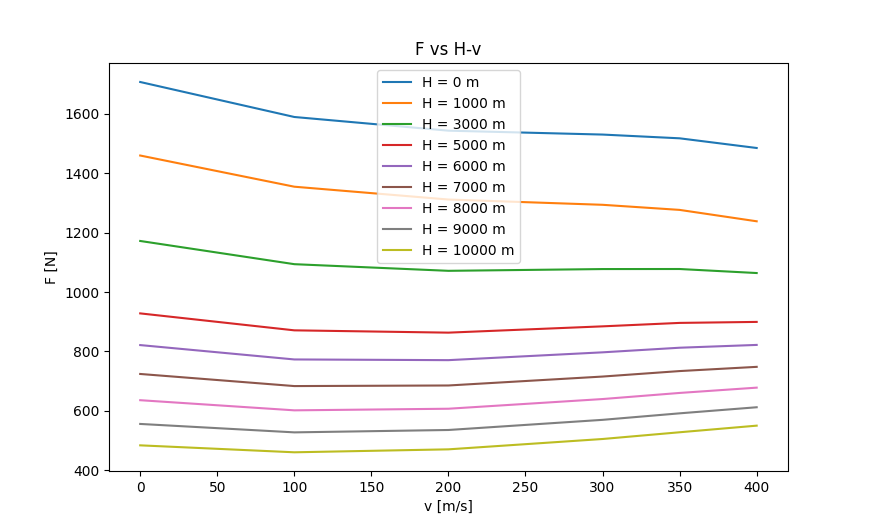
\includegraphics[width=\textwidth]{FHV.png}
  \caption{Thrust Performance with variation in speed and altitude}
  \label{fig:ThrustVar}
\end{figure}

\begin{figure}[h]
  \centering
  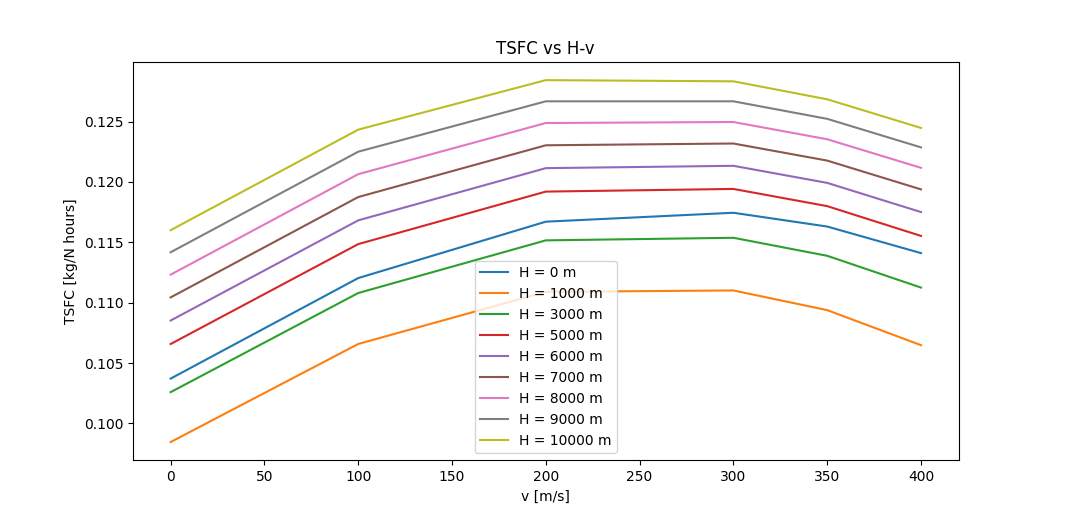
\includegraphics[width=\textwidth]{TSFCHV.png}
  \caption{TSFC with variation in speed and altitude}
  \label{fig:TSFCVar}
\end{figure}

\end{document}